\newpage
\textbf{\textcolor{MidnightBlue}{5.}}
Considera el algoritmo para calcular cortes consistentes visto en clase. Da una ejecución
para tres procesos en la que los canales de comunicación no son \code{FIFO} y el corte
calculado no es consistente.


\begin{center}
    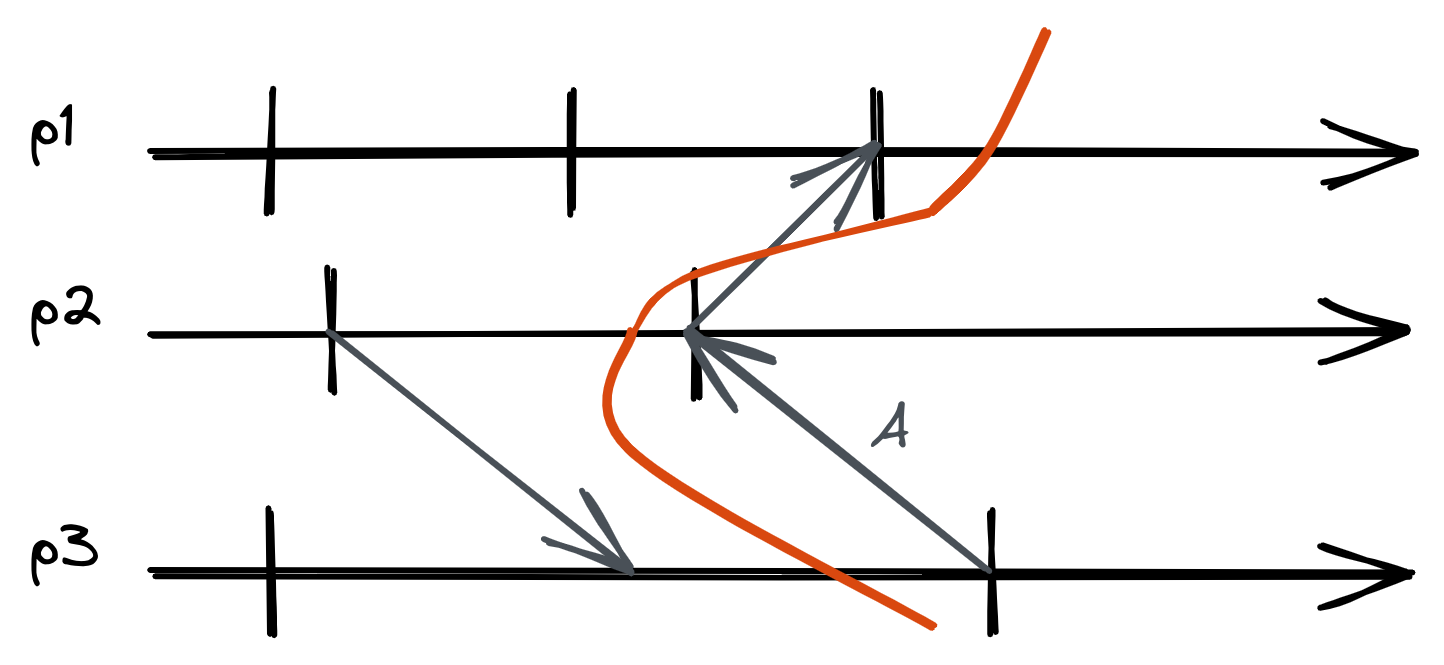
\includegraphics[width=\textwidth]{ejercicio5.png}
\end{center}

La siguiente ejecución no es \code{FIFO} dado que el mensaje con etiqueta \code{A} es recibido por el proceso A antes del mensaje que indicaría el corte. Notar que el siguiente corte (indicado por la linea naranja) no es consistente dado que el proceso 1 recibe un mensaje enviado por el proceso 2 el cual es un evento no contemplado en el corte. 